\cleardoublepage

\chapter[A friendly introduction to PCA]{A friendly introduction to principal component analysis}
\label{chapter:introduction}

We will work from the outside in: we will view PCA first as a way of finding a smaller representation of a dataset. This is a typical machine learning problem: find a compressed representation of the data such that the reconstructions are as close to the original as possible. This is a simple view of PCA, an we'll be able to compute it with nothing more than gradient descent with a few extra tricks for satisfying constraints.

Most of the technical stuff only becomes necessary when we want to understand why PCA works so well: this is where the \textbf{spectral theorem} and the \textbf{eigenvalues and -vectors}, come in to the story, they give us a deeper understanding of what we're doing. We'll look at these subjects in Chapter~\ref{chapter:eigenvectors}.

The spectral theorem is the heart of the method, so it pays to discuss it in some detail. We'll state it and explain what it means in Chapter~\ref{chapter:eigenvectors}, and leave the proof to Chapter~\ref{chapter:spectral-theorem}.

%Then, in Chapter~\ref{chapter:svd} we'll look at the the \textbf{singular value decomposition}. This matrix decomposition is not only the most popular method for computing the solutions to PCA, it is also the go-to method for computing many related problems, like least squares fits, and matrix ranks. Finally in Chapter

I'll assume some basic linear algebra knowledge, but  I'll try to explain the preliminaries where possible, even if they are fundamental to linear algebra. There is a small list of identities and properties in the appendix, which you may want to consult to refresh your memory. 

\section{The basics}

Let's begin by setting up some basic notation. We are faced with some high-dimensional dataset of instances (examples of whatever we're studying) described with real-valued features. That is, we have \(\gc{n}\) \emph{instances} \(\mbx_\gc{i}\) and each instance is described by a vector of \(\bc{m}\) real values. We describe the dataset as a whole as an \(\gc{n} \times \bc{d}\) matrix \(\mbX\) that is, we arrange the examples as rows, and the features as columns.

\begin{figure}[H]
	\centerline{
		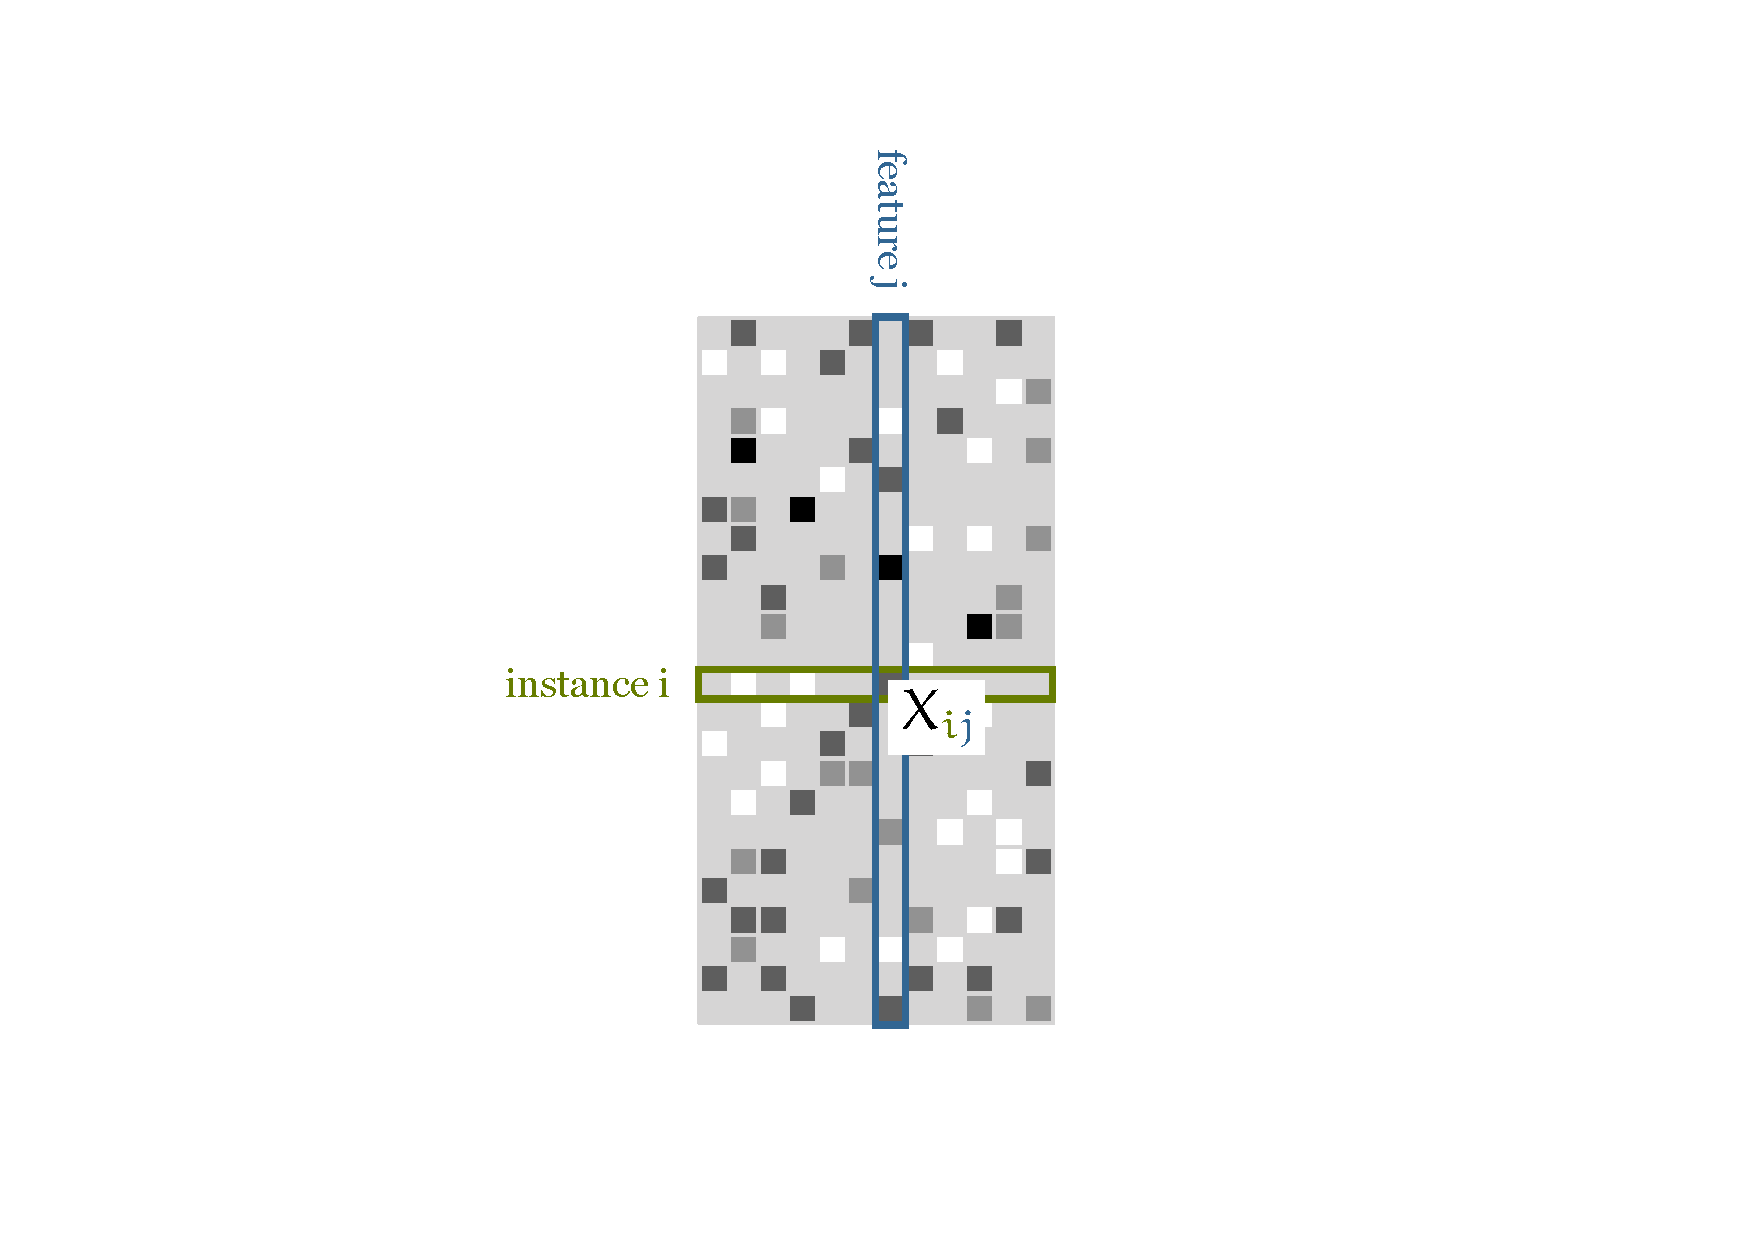
\includegraphics[width=0.6\textwidth]{./images/pca/data-diagram.pdf}
	}
\end{figure}

For a simple example, imagine that we have a dataset of \gc{100 people} with \bc{2 features} measured per person: their monthly salary and their income over the course of a quarter (i.e. three months). The second is just the first times 3, so this data is \emph{redundant}. One value can be computed from the other, so we really only need to store one number per person. Here's what that looks like in a scatterplot.

\begin{figure}[H]
	\centerline{
		\includesvg[width=\textwidth]{./images/pca/income1.svg}
	}
\end{figure}
\vspace{-2em}

\noindent Our intuition that we really only need one number to represent the data is reflected in the fact that \emph{the data form a line}. So long as we know what that line is, we only need to know how far along the line each instance is, so we can store the whole dataset in one number per instance.

\begin{aside}There are also more complex relations between two features that have this property, like a parabola or an exponential curve. In PCA we simplify things by only exploiting linear relations.	
\end{aside}

%
Of course, data in the wild is never this clean. Let's introduce some small variations between the monthly salary and the income after three months. Some people may have changed jobs, some people may get bonuses or vacation allowances, some people may have extra sources of income. Here's a more realistic version of the data.

\vspace{-2em}
\begin{figure}[H]
	\centerline{
		\includesvg[width=\textwidth]{./images/pca/income2.svg}
	}
\end{figure}

\noindent The data is no longer perfectly linear, but it still seems \emph{pretty} linear. If we imagine the same line we had in the last plot, and represent each person as a dot along that line, we lose some information, but we still get a decent \emph{reconstruction} of the data.

If you know how to do linear regression, you can probably work out how to draw such a line through the data, predicting the income from the salary or the other way around (and PCA is very similar to linear regression in many ways). However we'll need something that translates to higher dimensions, where we don't have a single target feature to predict.

\noindent To do so, we'll develop a method purely from these first principles:
\begin{enumerate}
\item We want to represent the data using a small set of numbers per instance.
\item We will limit ourselves to linear transformations of the data to derive this small set.
\item We want to minimize the error in our reconstruction of the data. That is, when we map the data back to the original representation, as best we can, we want it to be as close as possible to the original.
\end{enumerate}

\addvspace{2em}

\section{One-dimensional PCA} % ##
%
We'll develop a one-dimensional version of PCA first. That is, we will represent each instance \(\mbx_\gc{i}\) (row \(\gc{i}\) in our data matrix \(\mbX\)), by a single number \(z_\gc{i}\) as best we can. We will call \(z_\gc{i}\) the \emph{latent representation} of \(\mbx_\gc{i}\).

\begin{aside}The phrase ``latent'' comes from the Latin for \emph{being hidden}. This will make more sense when we see some of the other perspectives on PCA.
\end{aside}

\noindent To start with, we will assume that the data are \textbf{mean-centered}. That is, we have subtracted the mean of the data so that the mean of the new dataset is \(0\) for all features.

\vspace{-1em}
\begin{figure}[H]
	\centerline{
	\includesvg[width=0.9\textwidth]{./images/pca/mean-centered.svg}
	}
\end{figure}
\vspace{-2em}

%<figure class="narrow">
%<img src="/images/pca/mean-centered.svg" />
%</figure>
%
%<aside>
\begin{aside}
For now, think of this as a bit of necessary data pre-processing. We will see where this step comes from in the next chapter.
\end{aside}

Our task is to find a linear transformation from \(\mbx_\gc{i}\) to \(z_\gc{i}\), and another linear transformation back again.
%
A linear transformation from a vector \(\mbx_\gc{i}\) to a single number is just the dot product with a vector of weights. We'll call this vector \(\rc{\mbv}\). A linear transformation from a single number \(z_\gc{i}\) back to a vector is just the multiplication of \(z_\gc{i}\) by another vector of weights. We'll call this vector \(\rc{\mbw}\). This gives us
%
\begin{align*}
z_\gc{i} &= \rc{\mbv}^T \mbx_\gc{i} \\
\mbx'_\gc{i} &= z_\gc{i} \rc{\mbw}
\end{align*}
%
where \(\mbx'_\gc{i}\) is the reconstruction for instance \(\gc{i}\).

Look closely at that second line. It expresses exactly the intuition we stated earlier: we will choose one \rc{line}, represented by the vector \(\rc{\mbw}\), and then we just represent each data point by how far along the line it falls, or in other words, we represent \(\mbx'_\gc{i}\) as a multiple of \(\rc{\mbw}\).

\enlargethispage{3em}

\vspace{-1em}
\begin{figure}[H]
	\centerline{
	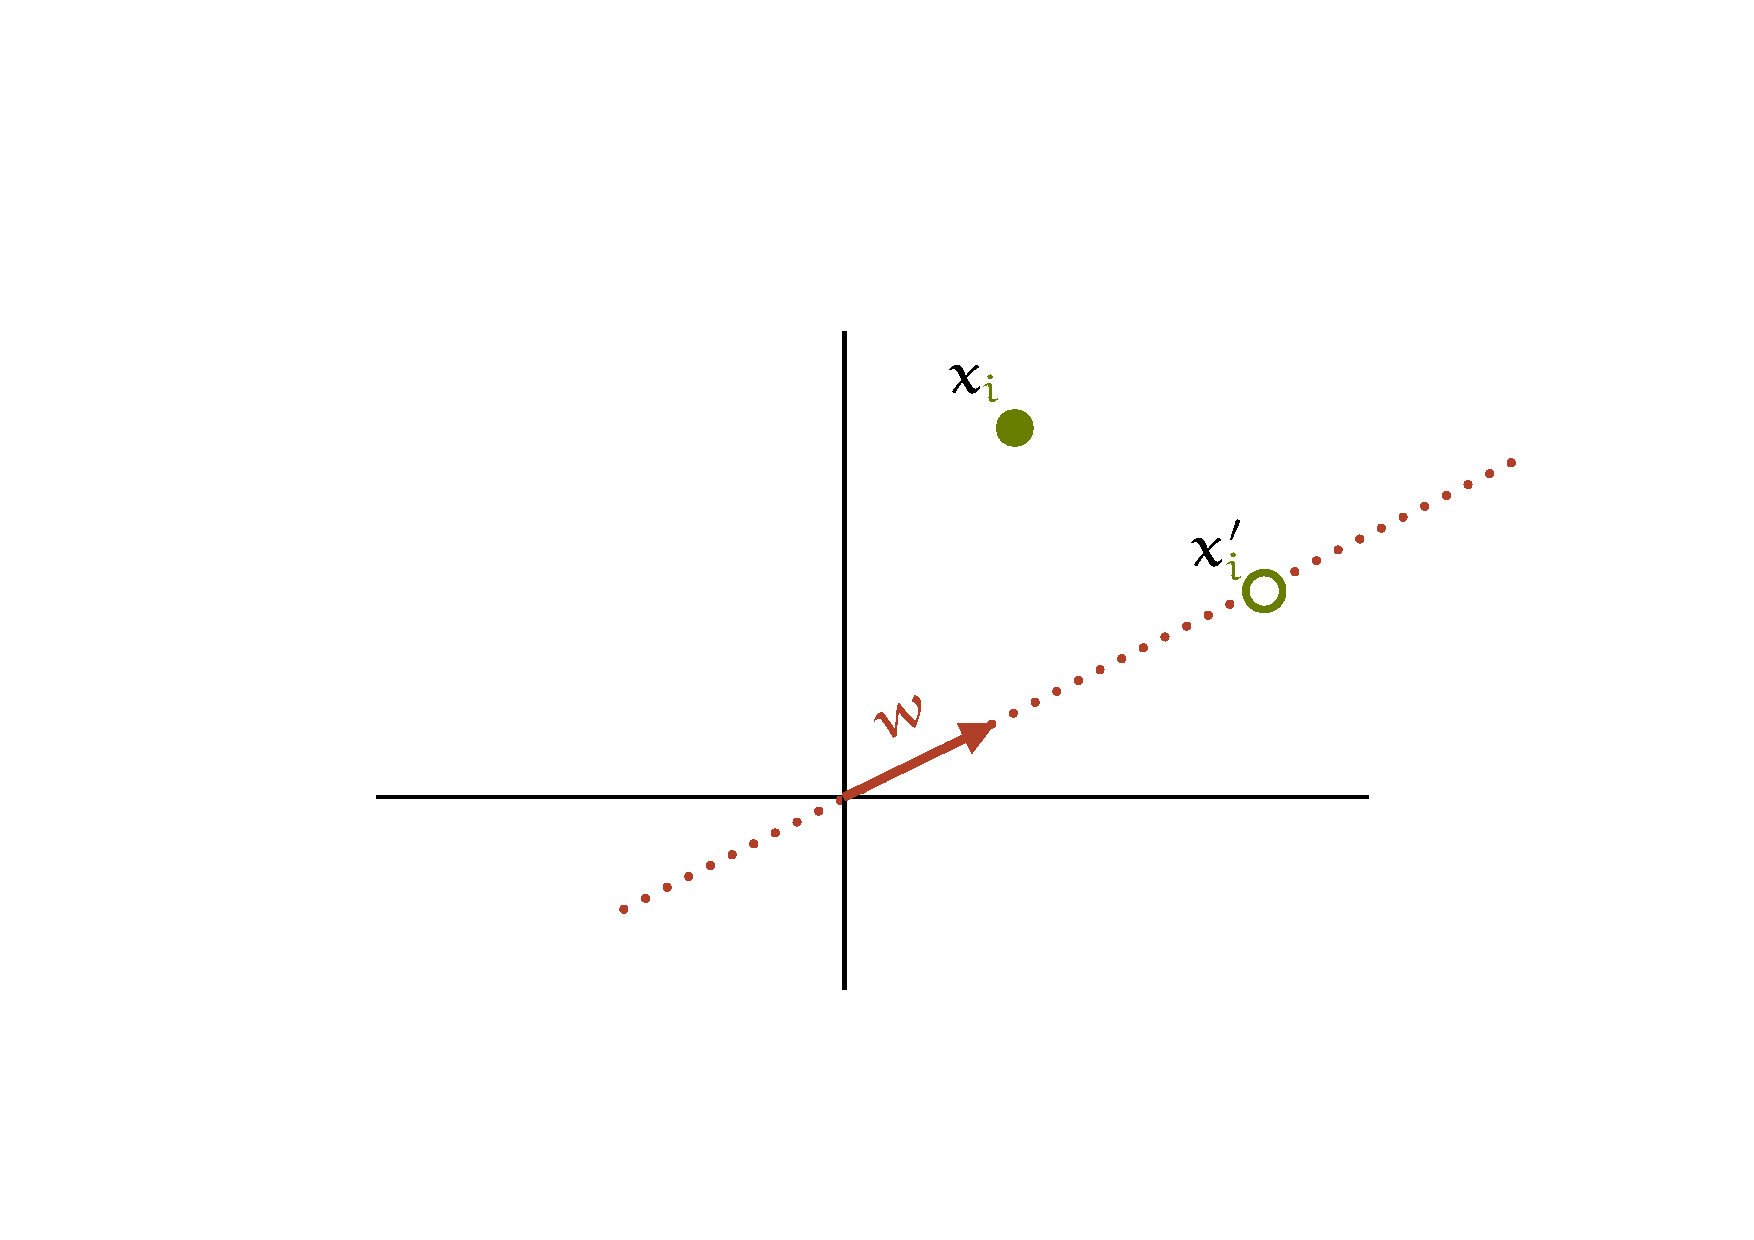
\includegraphics[width=0.8\textwidth]{./images/pca/projection.pdf}
	}
\end{figure}
\vspace{-1em}

%<figure class="narrow">
%<img src="/images/pca/projection.svg" />
%</figure>
%
\noindent All allowed values of \(\mbx'_\gc{i}\) are on the \rc{dotted red line}, which is defined by our choice of \(\rc{\mbw}\). Where each individual ends up is defined by the multiplier \(z_\gc{i}\), wich is determined by the weights \(\rc{\mbv}\). Our objective is to choose \(\rc{\mbv}\) and \(\rc{\mbw}\) so that the reconstruction error, the distance between \(\mbx_\gc{i}\) and \(\mbx'_\gc{i}\) is minimized (over all \(\gc{i}\)).

\vspace{-1em}
\begin{figure}[H]
	\centerline{
		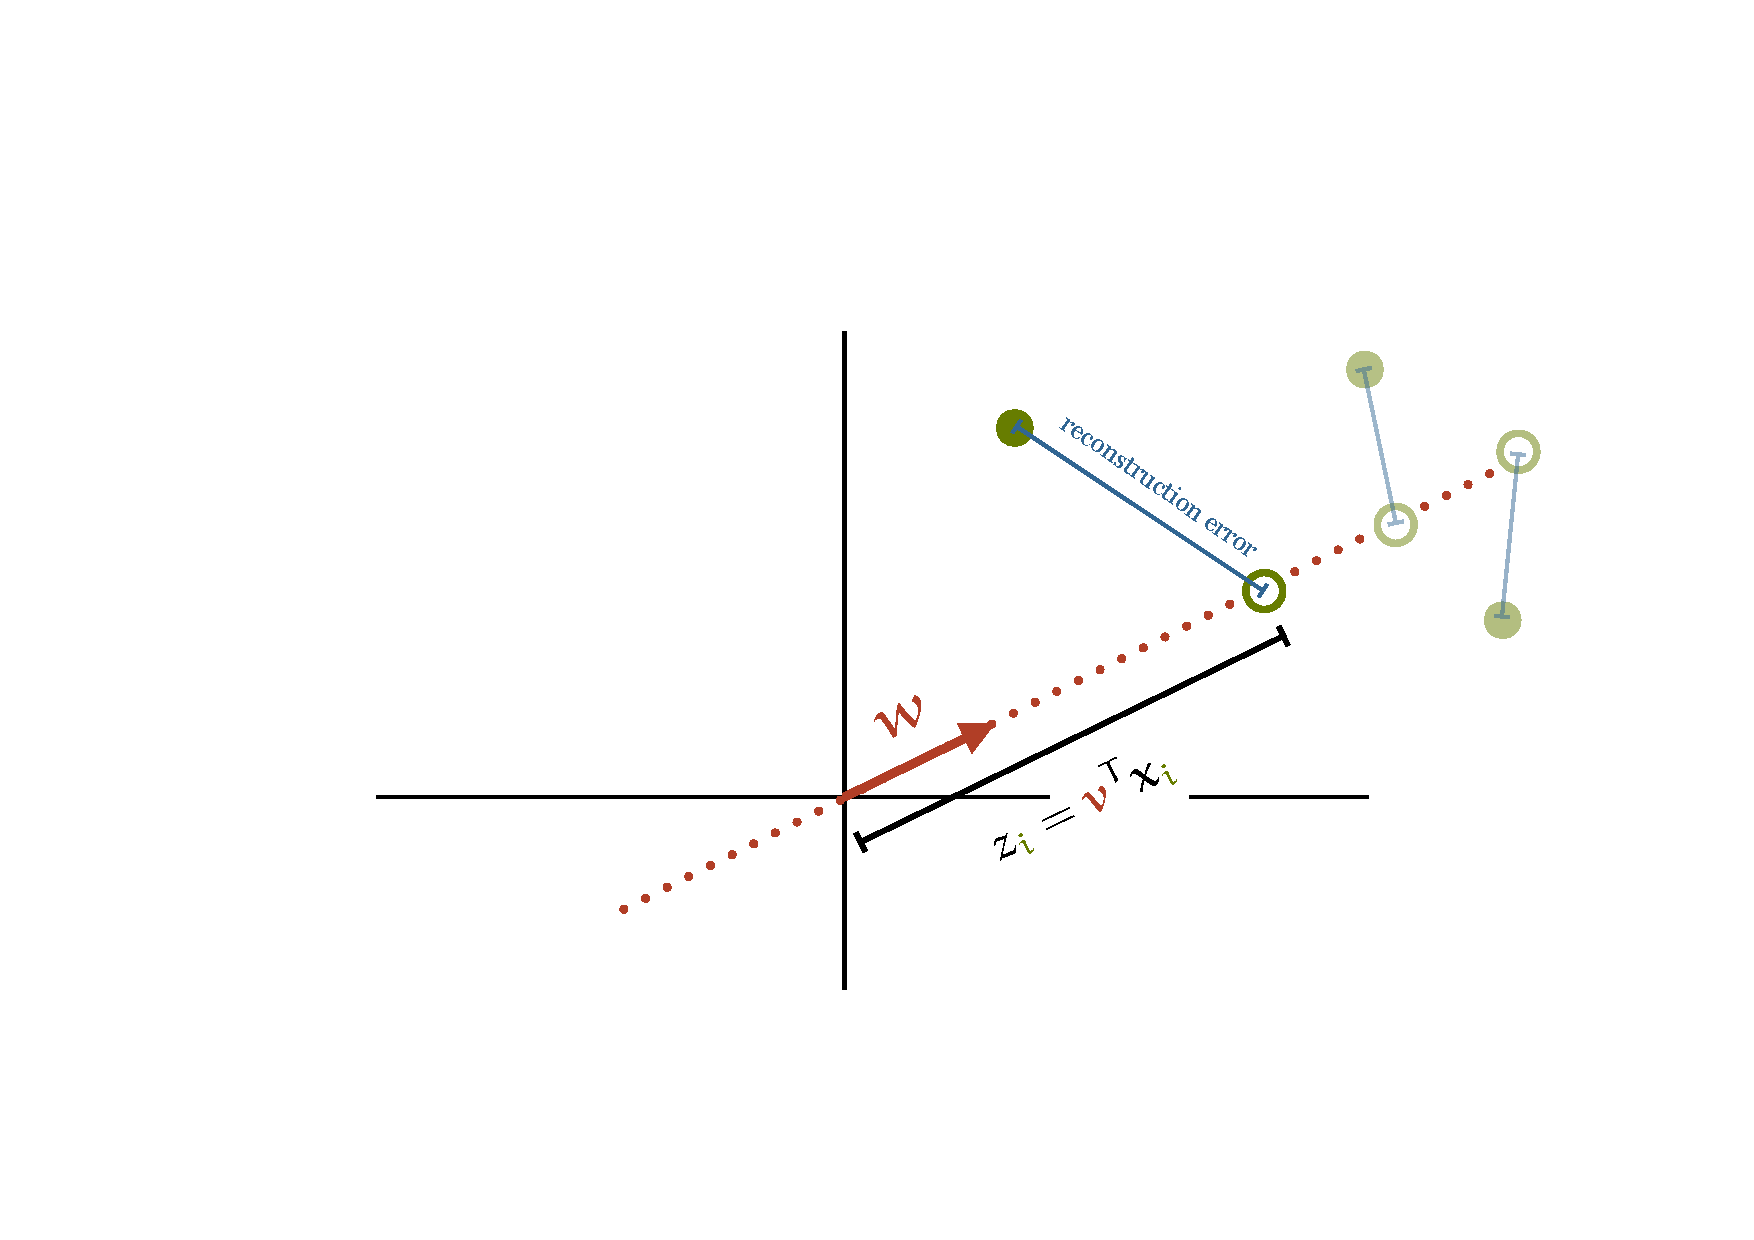
\includegraphics[width=0.8\textwidth]{./images/pca/reconstruction.pdf}
	}
\end{figure}
\vspace{-1em}

%<figure class="narrow">
%<img src="/images/pca/reconstruction.svg" />
%</figure>

\noindent We can simplify this picture in two ways. 

First, note that many different vectors \(\rc{\mbw}\) define the same \rc{dotted line} in the image above. So long as the vector points in the same direction, any length of vector defines the same line, and if we rescale \(z_\gc{i}\) properly, the reconstructed points \(\mbx'_\gc{i}\) will also be the same. To make our solution unique, we will \emph{constrain} \(\rc{\mbw}\) to be a unit vector. That is, a vector with length one: \(\rc{\mbw}^T\rc{\mbw} = 1\).

\begin{aside}
To be more precise, this doesn't leave a unique solution, but two solutions, assuming that a single direction is optimal, since the unit vector can point top right, or bottom left. In other words, if \(\rc{\mbw}\) is a solution, then so is \(-\rc{\mbw}\).
\end{aside}

The second simplification is that we can get rid of the second vector \(\rc{\mbv}\). Imagine that we have  some fixed \(\rc{\mbw}\) (that is, the \rc{dotted line} is fixed). Can we work out which choice of \(\mbx_\gc{i}\) on the line will minimize the \bc{reconstruction error}? We will go into a bit of detail here, since it helps to set up some intuitions that will be important in the later chapter of this book.

If you remember your linear algebra, you'll know that this happens when the line of the \bc{reconstruction error} is \emph{orthogonal} to the \rc{dotted line}. In more fancy language, the optimal \(\mbx_\gc{i}\) is the \emph{orthogonal projection} of \(\mbx_\gc{i}\) onto the dotted line. If you look at the image, it's not too difficult to convince yourself that this it true. You can imagine the reconstruction error as a kind of rubber band pulling on \(\mbx_\gc{i}\), and the point where it's orthogonal is where it comes to rest.

In higher dimensions, however, such physical intuitions will not always save us. Since the relation between orthogonality and least squares is key to understanding PCA, we will take some time to prove this properly.

\begin{theorem}[Best approximation theorem (1D)]
Let \(\rc{\mbw}, \mbx \in \mathbb{R}^n\),  let \(\rc{W}\) be the line of all multiples of \(\rc{\mbw}\), and let \(\rc{\hat \mbw}\) be the orthogonal projection of \(\mbx\) onto \(\rc{W}\). Then, for any other \(\rc{\bar \mbw}\) in \(\rc{W}\), we have 

\[
	\text{dist}(\mbx, \rc{\hat \mbw}) < \text{dist}(\mbx, \rc{\bar \mbw})
\]
where \(\text{dist}(\mba, \mbb)\) denotes the Euclidean distance \(\|\mba - \mbb\|\).
\end{theorem}
\begin{proof}[Adapted from Thm. 9 Ch. 7 in \cite{lay1994linear}] Note that \(\mba - \mbb\) is the vector that points from the tip of \(\mba\) to the bottom of \(\mbb\). We can draw three vectors \(\gc{\bar \mbw - \mbx}\), \(\bc{\hat\mbw -\mbx}\) and \(\rc{\bar \mbw - \hat \mbw}\) as follows:

%\vspace{-1em}

\begin{figure}[H]
	\centerline{
		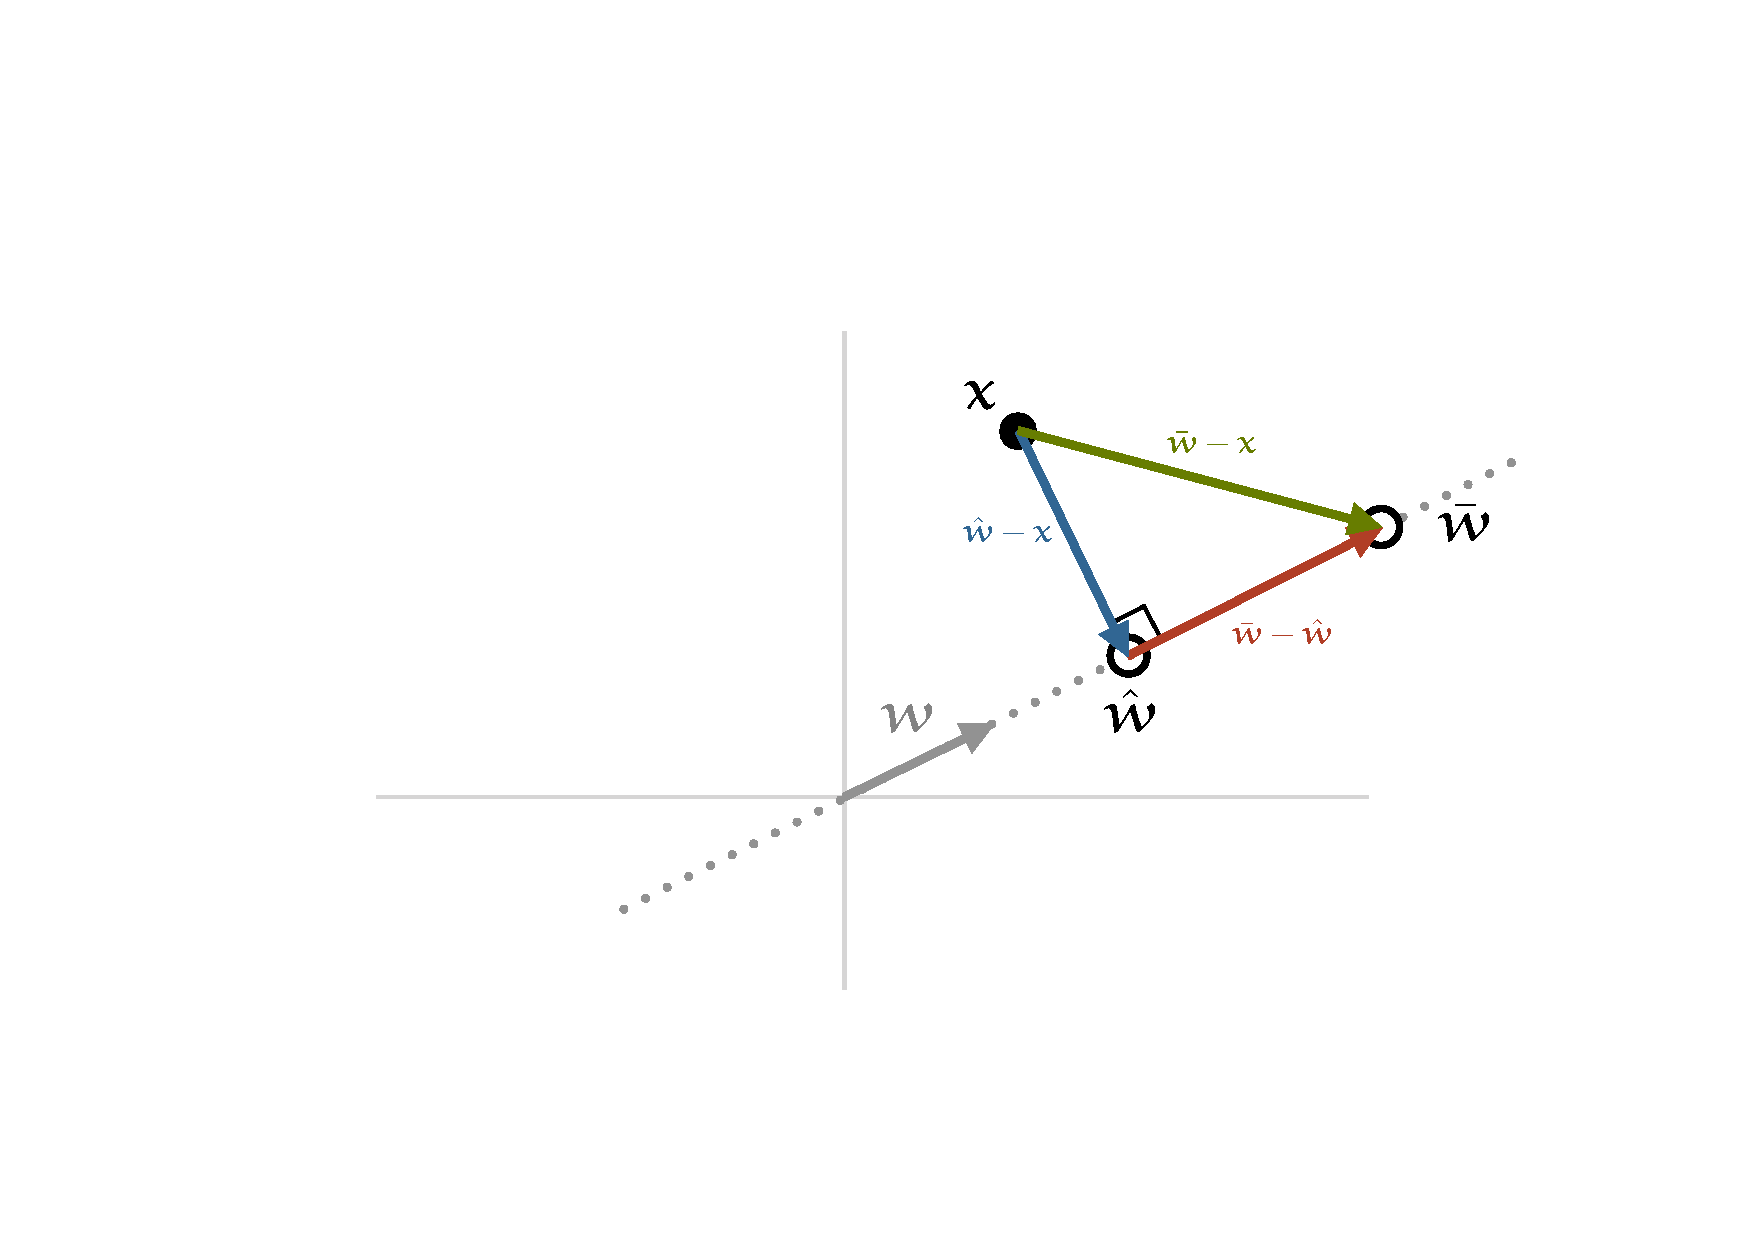
\includegraphics[width=1\textwidth]{./images/pca/pythagoras.pdf}
	}
\end{figure}
%
%\vspace{-1em}

%<figure class="narrow centering">
%<img src="/images/pca/pythagoras.svg" class="three-quarters"/>
%</figure>

By basic vector addition, we know that 

\[
\gc{\bar \mbw - \mbx} = \bc{\hat\mbw -\mbx} + \rc{\bar \mbw - \hat \mbw} \text{,}
\]

\textbf{so the three vectors form a triangle} (when we arrange them as shown in the picture).

We also know, by construction, that \(\bc{\hat\mbw -\mbx}\) is orthogonal to \(\rc{\bar \mbw - \hat \mbw}\), so \textbf{the triangle is right-angled}.

Since we have a right angled triangle, the Pythagorean theorem tells us that the lengths of the sides of the triangles are related by

\[
\gc{\text{dist}(\mbx, \bar \mbw)}^2 = \bc{\text{dist}(\hat \mbw, \mbx)}^2+ \rc{\text{dist}(\bar \mbw, \hat \mbw)}^2 \p
\]

Since \(\rc{\text{dist}(\bar \mbw, \hat \mbw)} > 0\) (because \(\bar \mbw\) and \(\hat \mbw\) are not the same point), we know that \(\gc{\text{dist}(\mbx, \bar \mbw)}\) must be strictly larger than \(\bc{\text{dist}(\hat \mbw, \mbx)}\). \hfill\qedsymbol
\end{proof}


\begin{aside}This result generalizes easily to any linear subspace \(\rc{W}\) spanned by a given set of vectors. We will show a more general proof in Chapter~\ref{chapter:svd}. This principle, the orthogonal projection as the best approximation is at the heart of a lot of optimization problems.
\end{aside}

So, the best reconstruction \(\mbx'_\gc{i}\) of the point \(\mbx_\gc{i}\) on the line defined by \(z \cdot \rc{\mbw}\) (however we choose \(\rc{\mbw}\)) is the orthogonal projection of \(\mbx_\gc{i}\) onto \(\rc{\mbw}\). So how do we compute an orthogonal projection? Let's look at what we have:

\vspace{-1em}
\begin{figure}[H]
	\centering
	\includesvg[width=1\textwidth]{./images/pca/projection2.svg}
\end{figure}
\vspace{-1em}

%<figure class="narrow centering">
%<img src="/images/pca/projection2.svg" class="three-quarters"/>
%</figure>

\noindent We've projected \(\mbx_\gc{i}\) down onto \(\rc{\mbw}\) and we've given the vector from the projection to the original the name \(\bc{\mbr}\). By vector addition we know that \(z\rc{\mbw} + \bc{\mbr} = \mbx_\gc{i}\), so \(\bc{\mbr} = \mbx_\gc{i} - z\rc{\mbw}\).


\pagebreak

\noindent Two vectors are orthogonal if their dot product is zero, so we're looking for a \(z\) such that \(z\rc{\mbw}^T\bc{\mbr} = 0\), or equivalently, \(\rc{\mbw}^T\bc{\mbr} = 0\). We rewrite

\[
0 = \rc{\mbw}^T\bc{\mbr} = \rc{\mbw}^T\left(\mbx_\gc{i} - z\rc{\mbw}\right) = \rc{\mbw}^T\mbx_\gc{i} - z\rc{\mbw}^T\rc{\mbw} \p
\]

This gives us \(z = \rc{\mbw}^T\mbx_\gc{i} / \rc{\mbw}^T\rc{\mbw}\). And, since we'd already defined \(\rc{\mbw}\) to be a unit vector (so \(\rc{\mbw}^T\rc{\mbw} = 1\)), we get \(z = \rc{\mbw}^T\mbx_\gc{i}\).

Let's retrace our steps. We had two weight vectors: \(\rc{\mbv}\) to encode \(\mbx_\gc{i}\) into the single number \(z_\gc{i}\), and \(\rc{\mbw}\) to decode \(\mbx_\gc{i}\) as \(z_\gc{i}\rc{\mbw}\). We've now seen that for any given \(\rc{\mbw}\), the best choice of \(z_\gc{i}\) is \(\rc{\mbw}^T\mbx_\gc{i}\). In other words, \textbf{we can set \(\rc{\mbv}\) equal to \(\rc{\mbw}\) and use it to encode and to decode}.

\begin{aside}
Note that an important requirement for this result (and its generalizations coming up) is  that \(\rc{\mbw}\) is a unit vector.
\end{aside}

So, after all that, we can finally state precisely what we're looking for. Given \(\rc{\mbw}\) our reconstruction is \(\mbx'_\gc{i} = z_\gc{i} \cdot \rc{\mbw} = \oc{\mbw^T\mbx_i \cdot \mbw}\). This means we can state our goal as the following constrained optimization problem:

\begin{align*}
&\argmin{\rc{\mbw}} \sum_\gc{i} \| \oc{\mbw^T\mbx_i \cdot \mbw}  - \mbx_\gc{i} \| \\
&\;\;\;\;\text{such that } \rc{\mbw}^T\rc{\mbw} = 1 \p
\end{align*}

How do we solve this? This is a simple problem and there are fast ways to solve it exactly. But we've done a lot of math already, and it's time to show you some results, so we'll just solve this by gradient descent for now. Basic gradient descent doesn't include constraints, but in simple cases like these, we  can use \emph{projected} gradient descent: after each gradient update, we project the parameters back to the subset of parameter space that satisfies the constraint (in this case simply by dividing \(\rc{\mbw}\) by its length).

\begin{aside}If you don't know \href{https://mlvu.github.io/lecture02/}{how gradient descent works}, you can just imagine a procedure that starts with a random choice for \(\rc{\mbw}\) and takes small steps in the direction that the function above decreases the most.
\end{aside}

We start by initializing \(\rc{\mbw}\) to some arbitrary direction. Here's what the projections of the income data onto that \(\rc{\mbw}\) look like.

%\vspace{-1em}
\begin{figure}[H]
	\centerline{
	\includesvg[width=0.899\textwidth]{./images/pca/random-w.svg}
	}
\end{figure}
%\vspace{-1em}

%<figure class="narrow">
%<img src="/images/pca/random-w.svg" />
%</figure>

The (squared) sum of the lengths of the \bc{blue lines} is what we want to minimize. Clearly, there are better options than this choice of \(\rc{\mbw}\). After a few iterations of gradient descent, this is what we end up with.

%\vspace{-1em}
\begin{figure}[H]
	\centerline{
	\includesvg[width=0.899\textwidth]{./images/pca/sol-w.svg}
	}
\end{figure}
%\vspace{-1em}

You can think of the blue lines of the reconstruction error as pulling on the line of \(\rc{\mbw}\) and of \(\rc{\mbw}\) as pivoting on the origin.
\pagebreak 

\noindent For any dataset (of however many dimensions), there is a unique, optimal line \(\rc{\mbw}\). It's called the \textbf{first principal component}.

\begin{aside}
If you've read other descriptions of PCA, you may be wondering at this point why I'm not talking about maximizing the variance. This is an alternative way to define PCA. We'll discuss it in the next chapter.
\end{aside}

What can we say about the meaning of the elements of \(\rc{\mbw}\)? Remember that it does two things: it encodes from \(\mbx\) to \(z\) and it decodes from \(z\) to \(\mbx'\). The encoding is a dot product: a weighted sum over the elements of \(\mbx\).

In the first example of the income data, before we added the noise, the second feature was always exactly three times the first feature. In that case, we could just remember the first feature, and forget the second. That would be equivalent to encoding with the vector \(\rc{(1, 0)}\). The compressed representation \(z\) would be equivalent to the first feature and we could decode with \(z \times\rc{(1, 3)}\). Or, we could encode with \(\rc{(0, 1)}\) and decode with \(\rc{(\tfrac{1}{3}, 1)}\).

Why are the encoding and decoding vectors different in these cases? Because when we proved that they were the same, we assumed that they were unit vectors. Our encoding vector is a unit vector, but the corresponding decoding vector isn't. PCA provides solution for which the encoder and the decoder are the same. It takes a mixture of both features, in different proportions (in our case \(1/\sqrt{10}\) and \(3/\sqrt{10}\)) . There are a a lot of perspectives on exactly what this mixture means. We'll illustrate the first by looking at a higher dimensional dataset.

We'll use a dataset of grayscale images of faces produced by AT\&T Laboratories Cambridge called the \emph{Olivetti dataset}.\footnotemark 

\footnotetext{\url{https://scikit-learn.org/stable/datasets/real_world.html\#the-olivetti-faces-dataset}}

\begin{figure}[t]
	\centerline{
	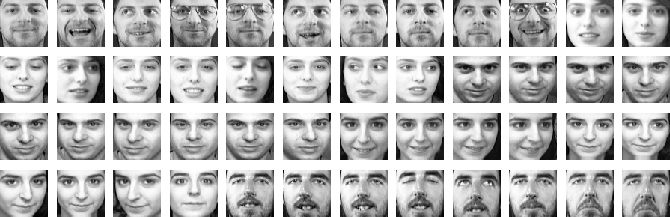
\includegraphics[width=1.2\textwidth]{./images/pca/faces.png}}
	\caption*{A small sample of images from the Olivetti data.}
\end{figure}
%\vspace{-1em}

%<figure class="narrow">
%<img src="/images/pca/faces.png" />
%</figure>

We will describe each pixel as a feature with a value between 0 (black) and 1 (white). The images are \(64 \times 64\) pixels, so each image can be described as a single vector of \bc{\(4096\) real values}.

\begin{aside}Note that by flattening the images into vectors we are entirely ignoring the grid structure of the features: we are not telling our algorithm whether two pixels are right next to each other, or at opposite ends of the image.
\end{aside}

The Olivetti data contains \gc{400 images}, so we end up with a data matrix \(\mbX\) of 
\(\gc{400} \times \bc{4096}\). 

\begin{figure}[H]
	\centering
	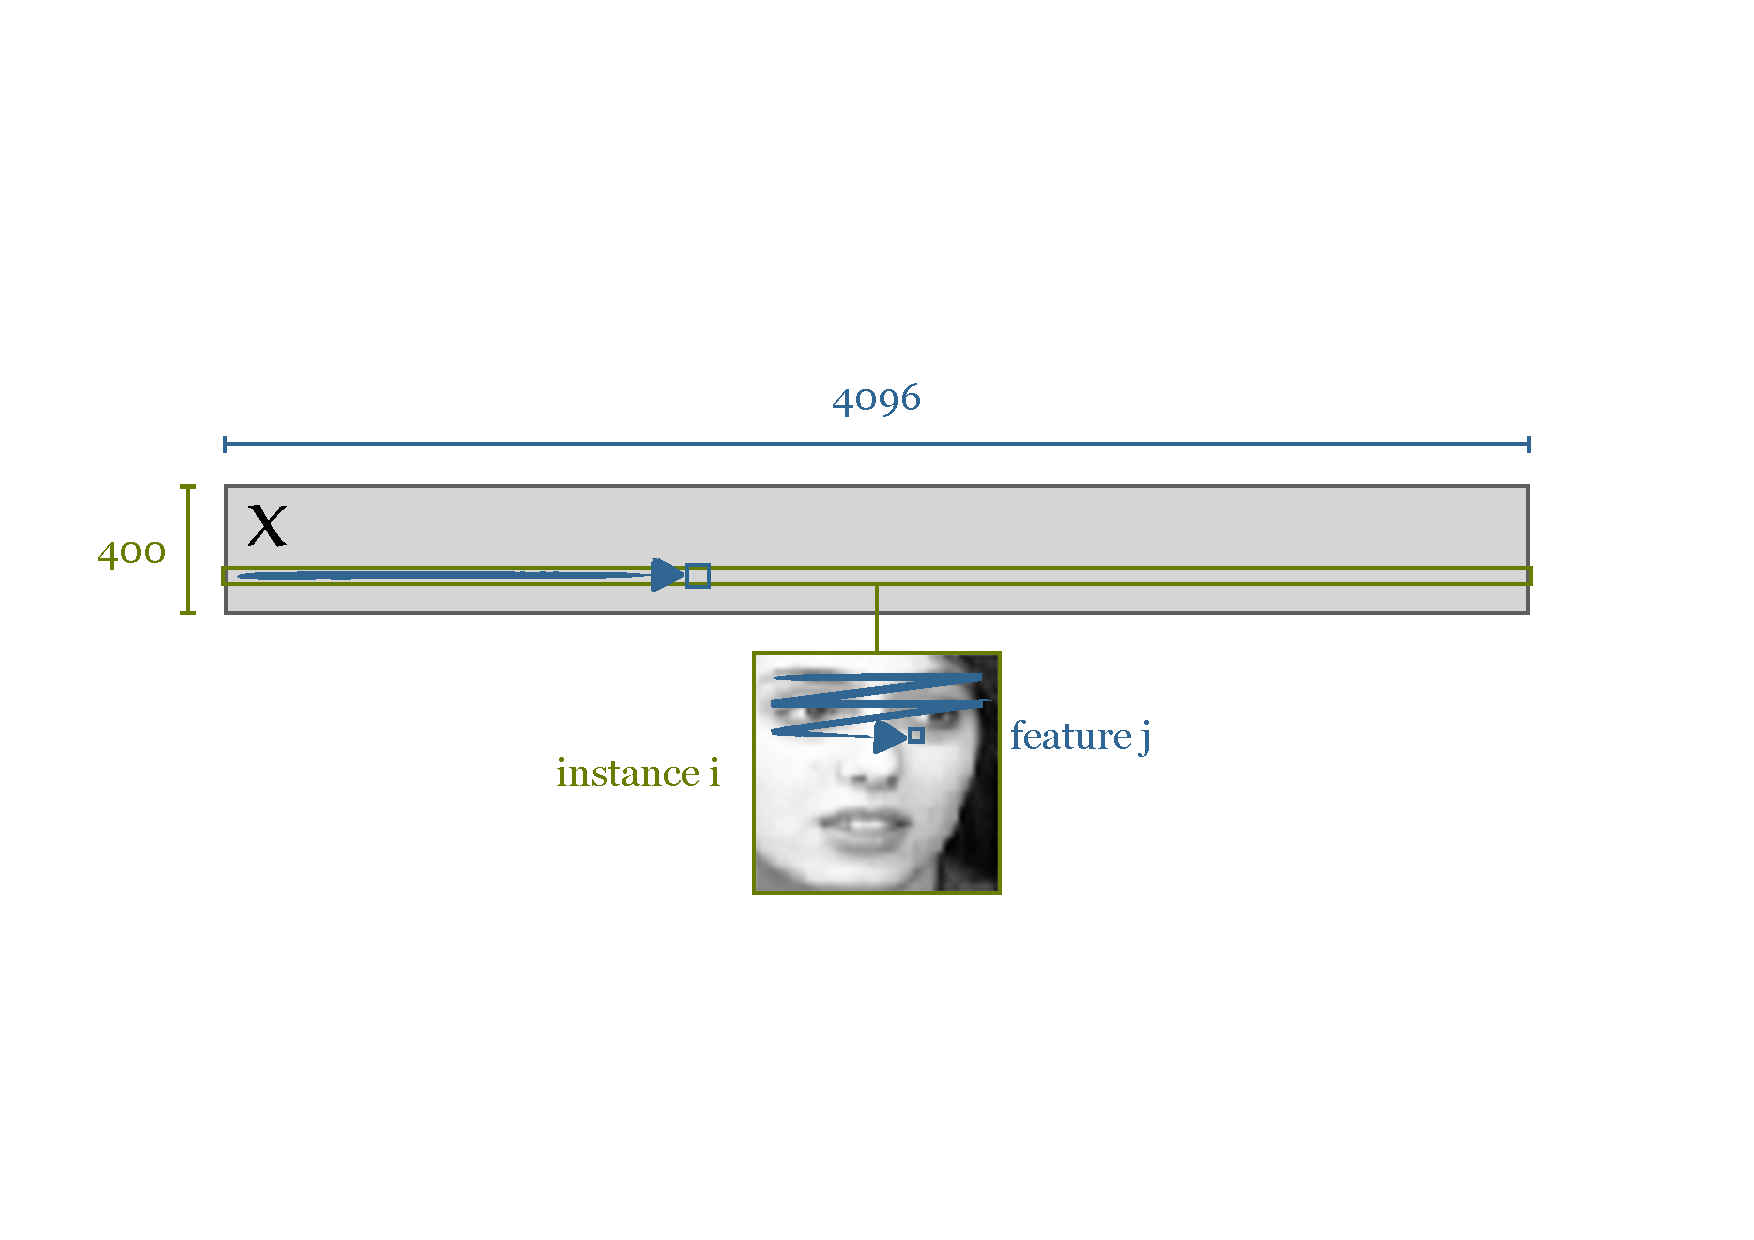
\includegraphics[width=1\textwidth]{./images/pca/images-diagram.pdf}
\end{figure}

%<figure class="narrow">
%<img src="/images/pca/images-diagram.svg" />
%</figure>

This is a data scientist's worst nightmare: data with many more features than instances. With so many features, the space of possible instances is vast, and we only have a tiny number to learn from. Our saving grace is that, like the income/salary example, the features in this dataset are highly \emph{dependent}: knowing the value of one pixel allows us to say a lot about the value of other pixels. 

For instance, pixels that are close together more often than not have similar values. The images are often roughly symmetric. All faces will have mostly uniform patches of skin in roughly the same place, and so on. 

In short, while our dataset is expressed in \bc{4096} dimensions, we can probably express the same information in many fewer numbers, especially if we are willing to trade off a little accuracy for better compression.

The procedure we will use to find the first principal component for this data is exactly the same as before---search for a unit vector that minimizes the reconstruction loss---except now the instances have \bc{4096} features, so \(\rc{\mbw}\) has \bc{4096} dimensions. First, let's look at the reconstructions.

\begin{figure}[H]
	\centerline{
	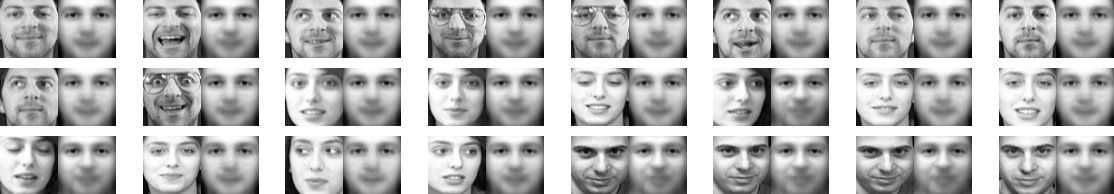
\includegraphics[width=1.4\textwidth]{./images/pca/face-reconstructions.png}
	}
	\caption*{Reconstruction from a single principal component. Originals on the left, reconstructions on the right.}
\end{figure}

%<figure class="wide-margin">
%<img src="/images/pca/face-reconstructions.png"/>
%</figure>

These are not very impressive yet, but to be fair, we've compressed each image into a single number, we shouldn't be surprised that there isn't much left after we reconstruct it. But that doesn't mean that 1D PCA doesn't offer us anything useful. 

What we can do is look at the first principal component in data space: \(\rc{\mbw}\) is a vector with one element per pixel, so we can re-arrange it into an image and see what each element in the vector tells us about the original pixels of the data. We'll color the positive elements of \(\rc{\mbw}\) red and the negative values blue.

\enlargethispage{4em}

It looks like this:

\begin{figure}[H]
	\centering
	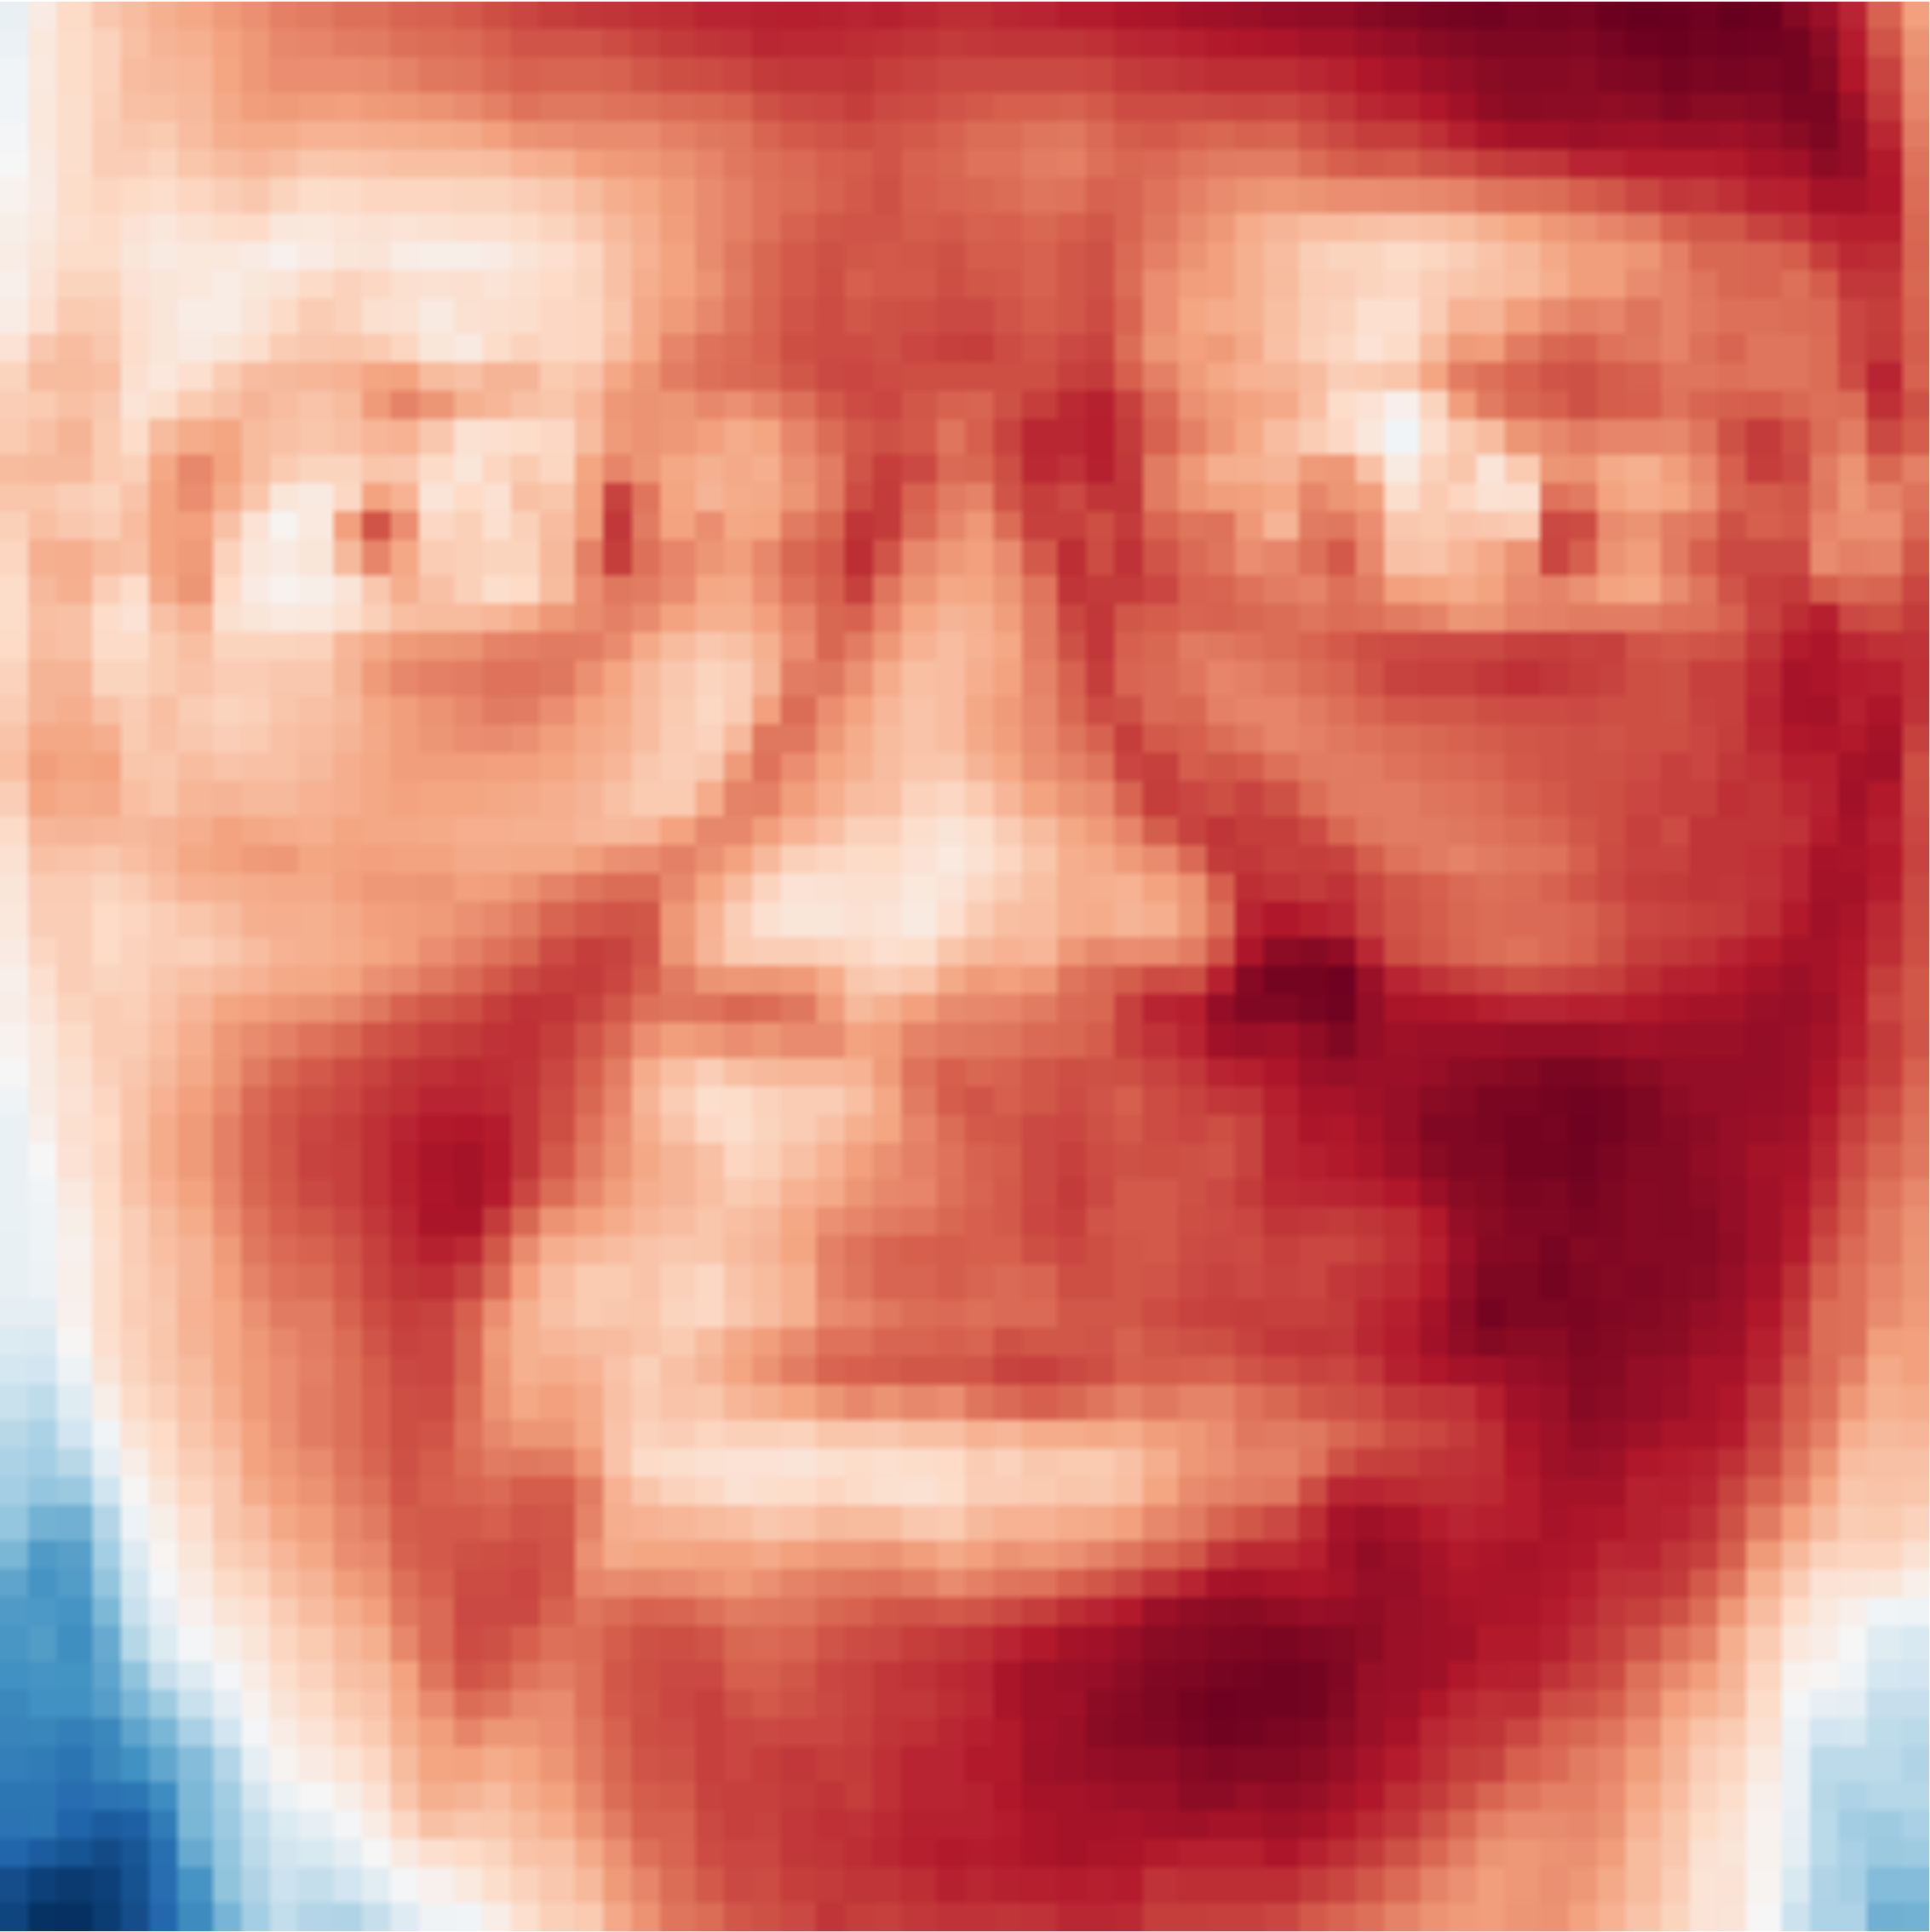
\includegraphics[width=0.4\textwidth]{./images/pca/firstpc.png}
\end{figure}

\noindent If we think of this as the \emph{encoding} vector, we can see a heatmap of which parts of the image the encoding looks at: the darker the red, the more the value of that pixel is added to \(z\). The darker the blue, the more it is subtracted. 

If we think of this as the \emph{decoding} vector, we can see that the larger \(z\) is, the more of the red areas gets added to the decoded image, but the more of the blue areas get \emph{subtracted}. That is, two red pixels are positively correlated, and a red and a blue pixel are negatively correlated. A bright red pixel and a light red pixel have the same relation as our monthly salary and quarterly income: one is (approximately) a multiple of the other.

%\begin{aside}
%If you rerun the code yourself, you may get the same images with blues and reds reversed. Remember that there are two solutions, one the negative of the other.
%\end{aside}

Another interpretation of the principal component is that it places the images in the dataset on a single line, which mean it orders the images along a single direction.

To see if there's any interpretable meaning to this ordering, we can try moving along the line and decoding the points we find. We can start at the origin (the vector \(\mathbold 0\)). If we decode that, we get the mean of our dataset (the so called mean face). By adding or subtracting a little bit of the principal component, we can see what happens to the face.

\begin{figure}[H]
	\centerline{
	\includesvg[width=1.2\textwidth]{./images/pca/int-mean-face.svg}
	}
\end{figure}

%<figure class="wide-margin">
%<img src="/images/pca/int-mean-face.svg"/>
%</figure>

A few things are happening at once: the skin is becoming less clear, the lines in the face become more pronounced, the glasses become more pronounced and the mouth curves upward. Most of this is consistent with moving from a young subject to an old one. 

We can test this on the faces in our dataset as well; our principal component is a direction in the data space, so we can start with an image from our data, and take small steps in the direction of the principal component, or in the opposite direction.

\begin{aside}%
You can think of this as manipulating the single-number latent representation \(z\) by adding some small amount \(\epsilon\). If we decode such a point, we get \((z+\epsilon)\rc{\mbw} = z\rc{\mbw} + \epsilon\rc{\mbw} = \mbx' + \epsilon\rc{\mbw}\). We then just replace the reconstruction \(\mbx'\) by the actual point \(\mbx\). Note that we depend on the linearity of our transformation: for nonlinear variants of PCA, this trick won't work anymore.
\end{aside}

Here's what we get.

\begin{figure}[H]
	\centerline{
	\includesvg[width=1.2\textwidth]{./images/pca/int-data-faces.svg}
	}
\end{figure}

%<figure class="wide-margin">
%<img src="/images/pca/int-data-faces.svg"/>
%</figure>

Note the manipulation of the mouth, in particular in face 41. As the corners of the mouth go up, the bottom lip goes from curving outward, with a shadow under the lip to curving inwards, folding under the teeth, with the shadow turning into a highlight.

\noindent Here we see the real power of PCA. While the reconstructions may not yet be much to write home about, the principal component itself allows us, using nothing but a linear transformation consisting of a single vector, to perform realistic manipulation of facial data, based on a dataset of just 400 examples.

\section{n-Dimensional PCA}

Enough playing around in a one-dimensional latent space. What if we want to improve our latent representations by giving them a little more capacity? How do we do that in a way that gives us better reconstructions, but keeps the meaningful directions in the latent space? 

Let's start by updating our notation. \(\mbx_\gc{i}\) is still the same vector, row \(\gc{i}\) in our data matrix \(\mbX\), containing \(\bc{m}\) elements, as many as we have features. \(\mbz_\gc{i}\) is now also a vector (note the boldface). \(\mbz_\gc{i}\) has \(\rc{k}\) elements, where \(\rc{k}\) is the number of latent features, a parameter we set. In the example above, \(\rc{k}=1\). We'll drop the \(\gc{i}\) subscript to clarify the notation.

\noindent Let's say we set \(\rc{k}=2\). If we stick to the rules we've followed so far---linear transformations by unit vectors---we end up with the following task: find two unit vectors \(\rc{\mbw}_\rc{1}\) and \(\rc{\mbw}_\rc{2}\) and define \(\mbz = (z_\rc{1}, z_\rc{2})\) by \(z_\rc{1} = \mbx ^T\rc{\mbw}_\rc{1}\) and \(z_\rc{2} = \mbx^T \rc{\mbw}_\rc{2}\). Each latent vector gives us a reconstruction of \(\mbx\). We sum these together to get our complete reconstruction.

We can combine the two vectors \(\rc{\mbw_1}\) and \(\rc{\mbw_2}\) in a single matrix \(\rc{\mbW}\) (as its columns) and write

\begin{align*}
\mbz &= \rc{\mbW}^T\mbx \\
\mbx' &= \rc{\mbW}\mbz
\end{align*}

Or, in diagram form:

\vspace{-1.5em}
\begin{figure}[H]
	\centering
	\includesvg[width=0.4\textwidth]{./images/pca/multiplication-nd.svg}
\end{figure}
\vspace{-1.5em}

%<figure class="narrow centering">
%<img src="/images/pca/multiplication-nd.svg" class="half"/>
%</figure>

\noindent This would already work fine as a dimensionality reduction method. You can think of this as an autoencoder, if you're familiar with those. However, we can add one more rule to improve our reduced representation. \textbf{We will require that \(\rc{\mbw_2}\) is orthogonal to \(\rc{\mbw_1}\).}

\begin{aside}%
This decision is important, and has many useful consequences. We'll save those for later. For now, we'll just take it at face value.
\end{aside}

In general, each component \(\rc{\mbw}_r\) we add should be orthogonal to all components before it: for \(\rc{k} = 3\) we add another unit vector \(\rc{\mbw_3}\), which should be orthogonal to both \(\rc{\mbw_1}\) and \(\rc{\mbw_3}\).

We can summarize these constraints neatly in one matrix equation: the matrix \(\rc{\mbW}\), whose columns are our \(\rc{\mbw}\) vectors, should satisfy:

\[
\rc{\mbW}^T\rc{\mbW} = \mbI
\]
%
where \(\mbI\) is the \(\rc{k} \times \rc{k}\) identity matrix. This equation combines both of our constraints: unit vectors, and mutually orthogonal vectors. On the diagonal of \(\rc{\mbW}^T\rc{\mbW}\), we get the dot product of every column of \(\rc{\mbW}\) with itself (which should be \(1\) so that it is a unit vector) and off the diagonal we get the dot product of every column of \(\rc{\mbW}\) with every other column (which should be \(0\), so that they are orthogonal).

How do we find our \(\rc{\mbW}\)? The objective function remains the same: the sum of squared distances between the instances \(\mbx\) and their reconstructions \(\mbx'\). To satisfy the constraints, we can proceed in two different ways. We'll call these the \emph{combined} problem and the \emph{iterative} problem.

The \textbf{combined} problem is simply to add the matrix constraint above and stick it into our optimization function. This gives us 

\begin{align*}
&\argmin{\rc{\mbW}} \sum_\mbx \|\rc{\mbW}\rc{\mbW}^T\mbx - \mbx\|^2 \\
&\;\;\text{such that } \rc{\mbW}^T\rc{\mbW} = \mbI
\end{align*}

The \textbf{iterative} problem defines optima for the vectors \(\rc{\mbw_r}\) in sequence. We use the same one-dimensional approach as before, and we find the principal components one after the other. Each step we add the constraint that the next principal component should be orthogonal to all the ones we've already found.


\pagebreak 

\noindent To put it more formally, we choose each \(\rc{\mbw_1}, \ldots, \rc{\mbw_k}\) in sequence by optimizing

\[
\;\;\;\;\;\;\;\; \rc{\mbw_r} = \begin{cases} 
	&\argmin{\rc{\mbw}} \sum_\mbx \|\mbx^T\rc{\mbw} \times \rc{\mbw} - \mbx\|^2 \\
	&\;\;\;\;\;\;\text{such that } \rc{\mbw}^T\rc{\mbw} = 1, \\
	&\;\;\;\;\;\;\text{and } \rc{\mbw}^T\rc{\mbw_i} = 0 \text{ for } \rc{i} \in [1 \ldots \rc{r}-1]
\end{cases}
\]

These approaches are very similar. In fact, they're sometimes confused as equivalent in the literature. Let's look how they relate in detail.

The vector \(\rc{\mbw_1}\) defined in the iterative problem, is the same vector we found in the one-dimensional setting above: the first principal component. If the two problems are equivalent (i.e. they have the same set of solutions), this vector should always be one of the columns of \(\rc{\mbW}\) in the combined problem.

how that this isn't guaranteed, we can look at the case where \(\rc{k} = \bc{m}\). That is, we use as many \rc{latent features} as we have \bc{features in our data}. In this case, the first vector \(\rc{\mbw}\) returned by the iterative approach is still the first principal component, as we've defined it above. However, for the combined approach, we can set \(\rc{\mbW} = \mbI\) for a perfect solution: clearly the columns of \(\mbI\) are orthogonal unit vectors, and \(\rc{\mbW}\rc{\mbW}^T\mbx - \mbx = \mbI\mbI^T\mbx - \mbx = \mbx -\mbx = {\mathbold 0}\), so the solution is optimal.

In short, a solution to the combined problem may not be a solution to the iterated problem. What about the other way around, does solving the iterated problem always give us a solution to the combined problem? Certainly the vectors returned are always mutually orthogonal unit vectors, so the constraint is satisfied. Do we also reach a minimum? It turns out that we do.

\begin{theorem}[Optimality of the iterative approach]
A solution to the iterative problem is also a solution to the combined problem. 
\end{theorem}

We will prove this in the second chapter. For now, you'll have to take my word for it. The combined problem has a large set of solutions, and the iterative approach provides a kind of unique point of reference within that space. 

%\vspace{-1em}
\begin{figure}[H]
	\centering
	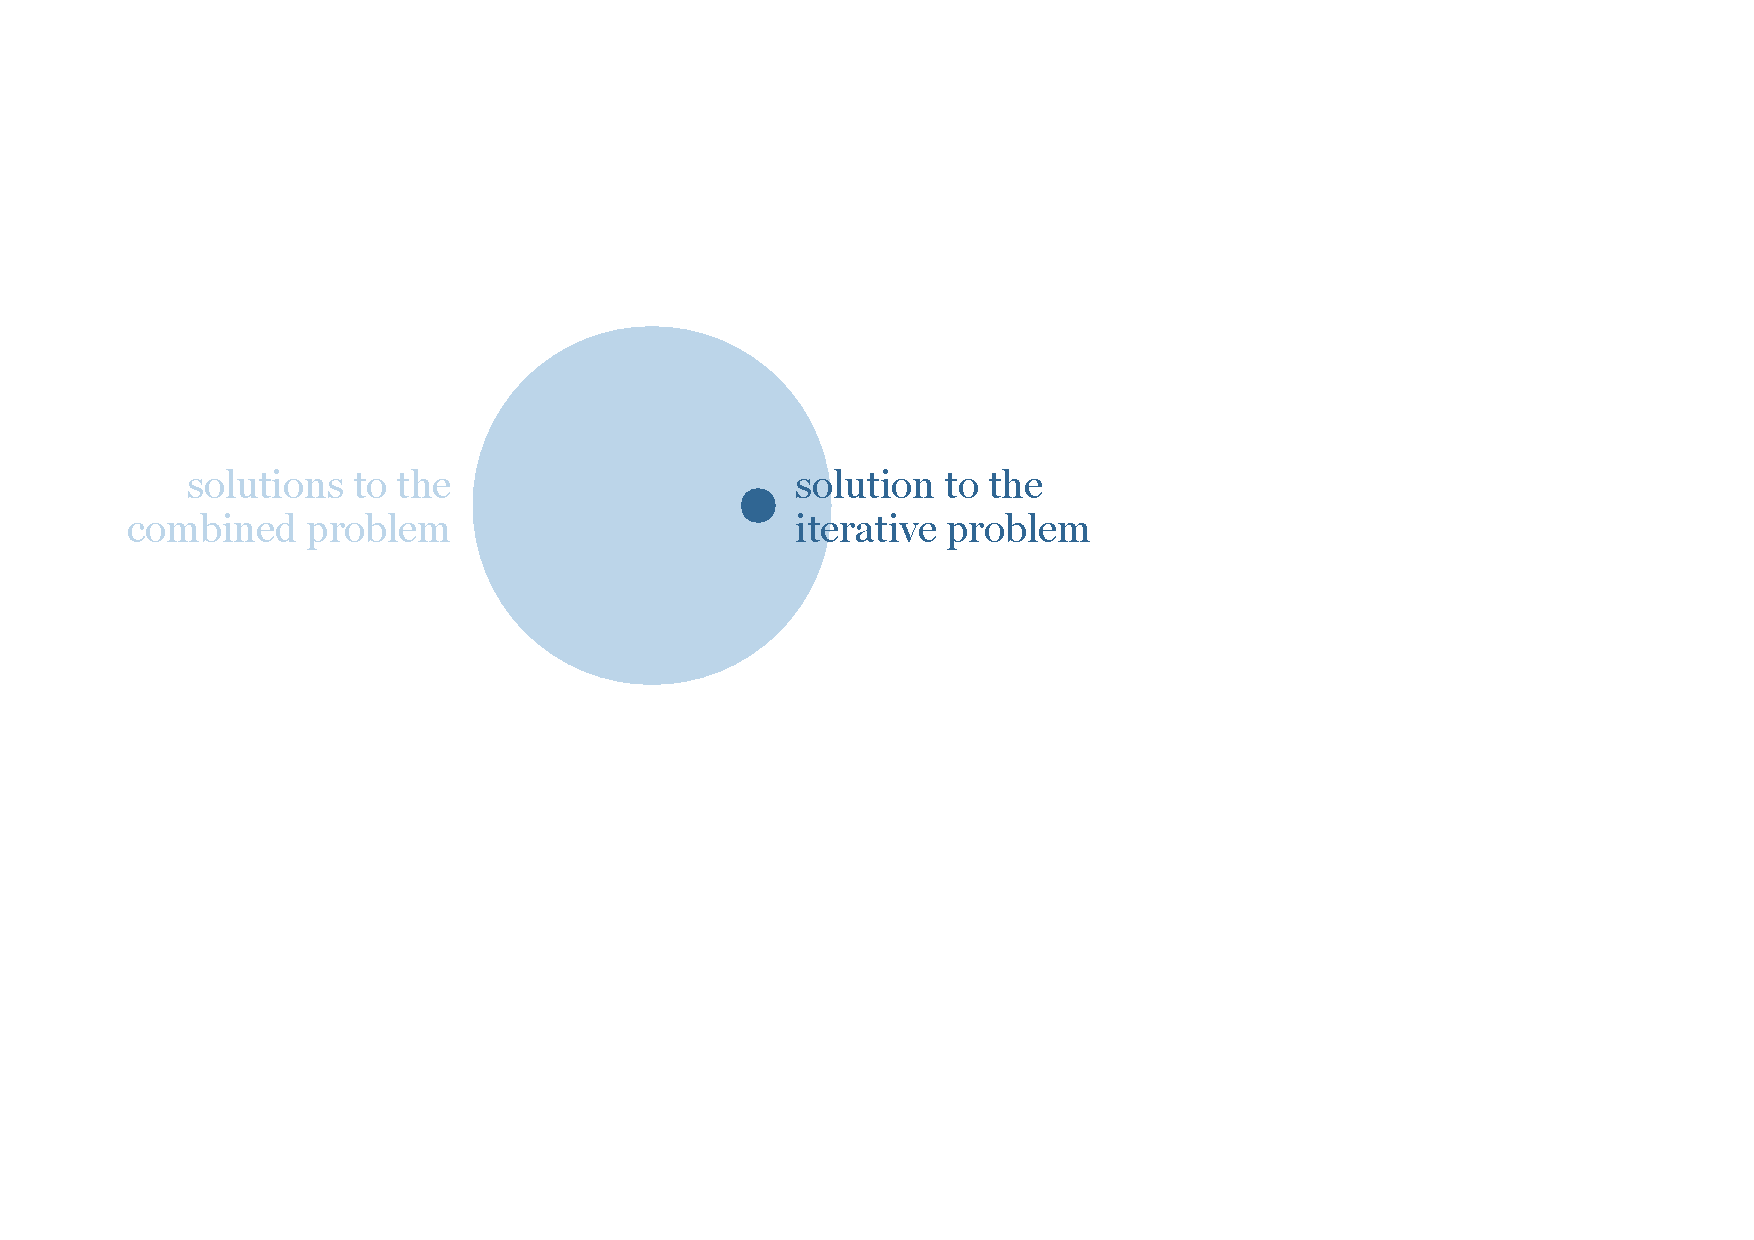
\includegraphics[width=0.8\textwidth]{./images/pca/venn.pdf}
\end{figure}
%\vspace{-1em}

%<figure class="narrow centering">
%<img src="/images/pca/venn.svg"/>
%</figure>

We can say more about this later, but for now we will equate the iterative solution with PCA: the \(\rc{\mbW}\) which not only minimizes the reconstruction error as a whole, but also each column of \(\rc{\mbW}\) minimizes the reconstruction error in isolation, constrained to the subspace orthogonal to the preceding columns. The combined problem does not give us the principal components.

Using the iterative approach, and solving it by projective gradient descent, we can have a look at what the other principal components look like. Let's start with our income data, and derive the second principal component.

\begin{figure}[H]
	\centering
	\includesvg[width=1\textwidth]{./images/pca/sol-w2.svg}
\end{figure}

This is a bit of an open door: in two dimensions, there is only one direction orthogonal to the first principal component. Still, plotting both components like this gives some indication of what the second component is doing. The first component captures the main difference between the people in our dataset: roughly their monthly salary. The second component captures whatever is left; all the noise we introduced like end of year bonuses and alternative sources of income.

Note how PCA reconstructs the original data points. Given the components \(\rc{\mbw_1}, \ldots, \rc{\mbw_k}\), we represent each \(\mbx\) as a weighted sum over these vectors where the latent features \(z_\rc{1}, \ldots, z_\rc{k}\) are the weights:

\[
\mbx' = z_\rc{1}\rc{\mbw_1} + z_\rc{2}\rc{\mbw_2}  + \ldots + z_\rc{k}\rc{\mbw_k}
\]

\begin{figure}[tb]
	\centering
	\includesvg[width=1\textwidth]{./images/pca/wsum.svg}
	\caption*{Reconstruction by principal components in the case where \(\rc{k}=3\). Each latent variable \(z_\rc{r}\) tells us how much of the \(\rc{r}\)-th principal component to add to our reconstruction.}
\end{figure}
%
%<figure class="narrow centering">
%<img src="/images/pca/wsum.svg"/>
%</figure>
%
That's it for the income dataset. We've reached \(\rc{k} = \bc{m}\), so we can go no further.

Let's turn to the dataset of faces, where there are many more principal components to explore.

If we compute the first 30 principal components, we get the following reconstructions.


\begin{figure}[H]
	\centerline{
	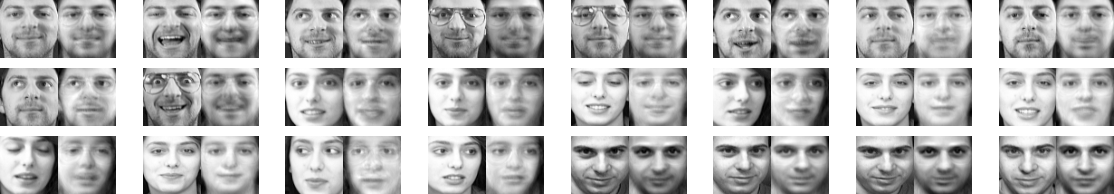
\includegraphics[width=1.2\textwidth]{./images/pca/face-reconstructions-k5.png}
	}
	
\end{figure}
%<figure class="wide">
%<img src="/images/pca/face-reconstructions-k5.png"/>
%</figure>

You can still tell the originals from the reconstructions, but many of the salient features now survive the compression process: the direction of the gaze, the main proportions of the face, the basic lighting, and so on. By looking at the first five principal components, we can see how this is done.

\begin{figure}[H]
	\centerline{
	\includesvg[width=1.2\textwidth]{./images/pca/five-pcs.svg}
	}
\end{figure}
%<figure class="narrow centering">
%<img src="/images/pca/five-pcs.svg"/>
%</figure>

The first one we've seen already. It's flipped around, this time, with the blues and reds reversed, but it defines the same line in space. Note that the magnitude of the higher PCs is much lower: the first principal component does most of the work of putting the image in the right region of space, and the more PCs we add, the more they fine-tune the details. 

The second PC captures mostly lighting information. Adding it to a picture adds to the left side of the image, and subtracts from the right side. We can see this by applying it to some faces from the data.

\begin{figure}[H]
	\centerline{
	\includesvg[width=1.2\textwidth]{./images/pca/int-data-faces-pc1.svg}
	}
\end{figure}
%<figure class="wide-margin">
%<img src="/images/pca/int-data-faces-pc1.svg"/>
%</figure>

The third PC does the same thing, but for top-to-bottom lighting changes. The fourth is a bit more subtle. It's quite challenging to tell from the plot above what the effect is. Here's what we see when we apply it to some faces.

\begin{figure}[H]
	\centerline{
	\includesvg[width=1.2\textwidth]{./images/pca/int-data-faces-pc3.svg}
	}
\end{figure}
%<figure class="wide-margin">
%<img src="/images/pca/int-data-faces-pc3.svg"/>
%</figure>

The PC seems to capture a lot of the facial features we associate with gender. The faces on the left look decidedly more "female", and the faces on the right more male. It's a far cry from the face manipulation methods that are currently popular, but considering that we have only 400 examples, we are only allowed a linear transformation, and that the method originated in 1901 \citep{pearson1901liii}, it's not bad.

\section{Applications of PCA}

Before we finish up, let's look at two examples of how PCA is used in research.
 
\noindent Let's start with a problem which crops up often in the study of fossils and other bones. A trained anatomist can look at, say, a shoulder bone fossil, and tell instantly whether it belongs to a chimpanzee (which is not very rare) or an early ancestor of humans (which is extremely rare). Unfortunately such judgements are usually based on a kind of unconscious instinct, shaped by years of experience, which makes it hard to back it up scientifically. "This is is Hominid fossil, because it looks like one to me," isn't a very rigorous argument. 

PCA is often used to turn such a snap judgement into a more rigorous analysis. We take a bunch of bones that are entirely indistinguishable to the layperson, and we measure a bunch of \bc{features}, like the distances between various parts on the bone. We then apply PCA and plot the first two principal components.

Here is what such a scatterplot looks like for a collection of scapulae (shoulder bones) of various great apes and hominids.

\begin{figure}[H]
	\centerline{
	\includesvg[width=1\textwidth]{./images/pca/bones.svg}
	}
\end{figure}

%<figure class="narrow">
%<img src="/images/pca/bones.svg"/>
%<figcaption>Reproduced from [4].</figcaption>
%</figure>

This particular figure is from \citet{young2015fossil} (reproduced with permission) which is \href{https://www.pnas.org/content/112/38/11829}{available online}, but the literature is full of images like these. Here, the authors took scans of about 350 scapulae. We can clearly see different species forming separate clusters. If we find a new scapula, we can simply measure it, project it to the first two principal components, and show that it ends up among the Homo Ergaster to prove that our find is special. What's more, not only can we tell the Hominin fossils apart, we see that they seem to lie on a straight line from chimpanzees to modern humans, giving a clue as to how human evolution progressed.

\begin{aside}%
This analysis is based on full 3D scans of the bones, but it also works if you measure a number of features by hand.
\end{aside}

Let's add one final example, to really hammer home the magic of PCA. When large-scale genome databases began to be gathered, one of the first things researchers did was to perform principal component analyses. 
To do so, all you need to do is to extract some features from the DNA sequence. This is easy enough to do: for instance, you can identify a few hundred thousand important genetic markers, and use the presence or absence of each as a binary feature.


\enlargethispage{3em}

\begin{figure}[H]
	\centerline{
	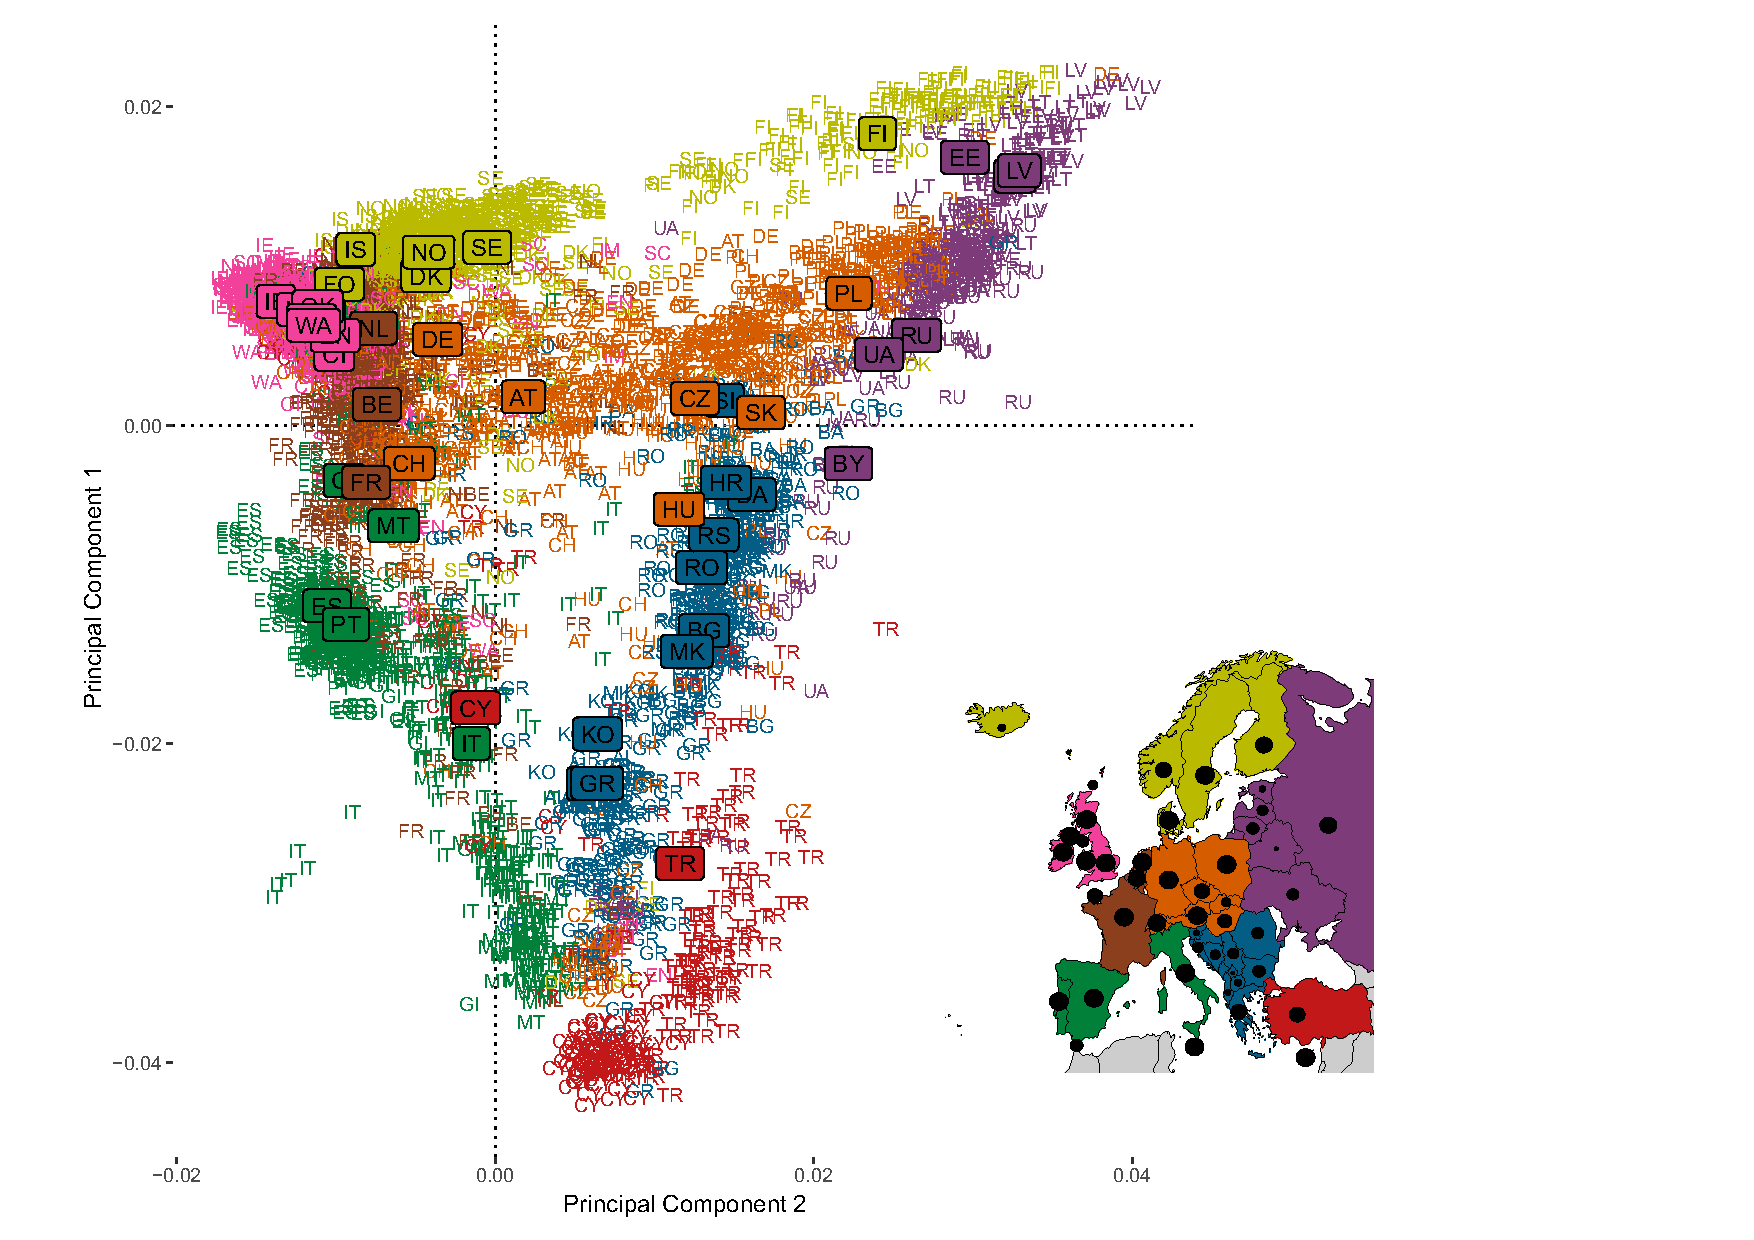
\includegraphics[width=0.7\textwidth]{./images/pca/europe-pnas.pdf}
	}
	\caption*{A PCA analysis of a European population, similar to the one by \cite{novembre2008genes}, colored by ancestry. Adapted from \cite{gilbert2022revealing}.
	}
\end{figure}

This was first done by \citet{novembre2008genes} for a dataset of 1387 Europeans, measuring about 200\,000 genetic markers. They applied PCA, and plotted the first two principal components. They then colored the instances by the person's ancestral country of origin (the country of origin of the grandparents if available, otherwise the person's own country of origin). What they saw was something like a blurry picture of Europe.

%  applied PCA to a database of 1387 European DNA sequences. For each instance, they measured about half a million sites on the DNA sequences to use as features. This is similar to the face example: many more features than instances.

%The authors applied PCA, and plotted the first two principal components. They colored the instances by the person's ancestral country of origin (the country of origin of the grandparents if available, otherwise the person's own country of origin). Here is what they saw.

%\begin{figure}[H]
%	\centerline{
%	\includesvg[width=0.9\textwidth]{./images/pca/europe.svg}
%	}
%\end{figure}

%<figure class="narrow">
%<img src="/images/pca/europe.svg"/>
%<figcaption>Reproduced from [5].</figcaption>
%</figure>

The first principal component corresponds roughly to how far north the person lives (or their ancestors did) and the second principal component to how far east they live. This means that a scatterplot shows up as a fuzzy map of Europe. If we sent a thousand DNA samples off to aliens on the other side of the galaxy, they could work out a rough image of the geography of Earth.

\begin{aside}%
Note that while this result is impressive, it's easy to misinterpret what this means. These to principal components together explain no more than a few percent of the variance. That is, while we can make a crude prediction of a person's origin from their DNA, we can predict almost nothing about their DNA from their origin. We saw something similar in the example of the Olivetti data: we could predict people's gender and age from the first few principal components, but when we reconstructed the photograph from just this information, the result removed almost all relevant details about the subject of the photograph.
\end{aside}


Wrapping up, what have we learned so far? We have defined PCA as an iterative optimization problem designed to compress high dimensional data into fewer dimensions, and to minimize the resulting reconstruction loss. We've shown one simple way to find this solution, a laborious and inaccurate way, but enough to get the basic idea across. We then looked at various practical uses of PCA: analyzing human faces, human fossils, and human DNA. We showed that in many cases, PCA magically teases out high-level semantic features hidden in the data: the species of the fossil, the location of the subject in Europe, or the subject's age.

What we haven't discussed fully, is where this magical property comes from. We've shown that it isn't \emph{just} the compression objective, since optimizing just that in one single optimization doesn't lead to the PCA solution. Among the set of all solutions that minimize the reconstruction error, the PCA solution takes a special place. Why that's the case, and why it this should emerge form optimizing the principal components one by one, greedily if you will, instead of all together, we will discuss in the next chapter. To do so, we'll need to dig into the subject of \emph{eigenvectors}, the underlying force behind almost everything that is magical about linear algebra.
